\documentclass{article}
\usepackage[margin=1in]{geometry}
\usepackage{amsmath}
\usepackage{amssymb}
\usepackage{amsthm}
\usepackage{bm}
\usepackage{hyperref}
\usepackage{graphicx}
\usepackage{caption}
\usepackage{listings}
\usepackage{xcolor}
\usepackage{float}
\usepackage{booktabs}
\usepackage{longtable}
\usepackage{multirow}
\usepackage{placeins}
\graphicspath{{figures/}}

% Code style
\lstdefinestyle{code}{
  basicstyle=\ttfamily\small,
  numbers=left,
  numberstyle=\tiny,
  numbersep=8pt,
  keywordstyle=\color{blue},
  commentstyle=\color{teal!70!black},
  stringstyle=\color{orange!70!black},
  showstringspaces=false,
  breaklines=true,
  frame=single,
  framerule=0.3pt,
  rulecolor=\color{black!15}
}
\lstset{style=code}

\title{Retrieval-Augmented Generation: Mechanics, Vector Infrastructure, and Fine-tuning Synergy}
\author{}
\date{\today}

\begin{document}
\maketitle

\section{Principles of Retrieval Augmentation and Knowledge Injection}
\subsection{Core concepts}
Retrieval-Augmented Generation (RAG) enriches language models with external knowledge bases to mitigate hallucinations and stale parameters. The pipeline in Figure~\ref{fig:rag_pipeline_en} depicts the standard flow: encode the query, retrieve top-$k$ candidates via vector search, fuse evidence into the prompt, and produce grounded answers with citations.
\begin{figure}[H]
  \centering
  
\includegraphics[width=0.9\textwidth]{rag_pipeline.png}
  \caption{RAG pipeline: embedding, vector search, context fusion, and grounded LLM generation.}
  \label{fig:rag_pipeline_en}
\end{figure}

\subsection{Retrieval-generation feedback loop}
\begin{itemize}
  \item \textbf{Bidirectional dependency:} Retrieval quality upper-bounds generation fidelity; generation instructions (citation format, answer structure) influence required context granularity.
  \item \textbf{Injection strategies:} Concatenate passages, craft structured prompts, rewrite queries, or apply re-ranking to prioritize authoritative evidence.
  \item \textbf{Adaptive control:} Incorporate failure handlers (e.g., “no answer” detection, query reformulation) and iterative retrieval to maintain accuracy.
\end{itemize}

\subsection{Architecture variants}
\begin{longtable}{p{3.2cm}p{5cm}p{6cm}}
\toprule
Variant & Description & Use cases \\
\midrule
Classic RAG & Query $\rightarrow$ retrieval $\rightarrow$ concatenation $\rightarrow$ generation & FAQ bots, knowledge base QA, domain chat assistants \\
Two-stage (ANN + rerank) & Vector retriever followed by cross-encoder reranking & Legal, medical, finance scenarios requiring high precision \\
Adaptive retrieval & LLM decides whether to retrieve, how often, and with which rewrite & Tool-augmented agents, real-time research assistants \\
Summarized documents & Pre-compute hierarchical summaries before retrieval & Long document reading, multi-report synthesis \\
\bottomrule
\end{longtable}

\section{Document Chunking and Embeddings}
\subsection{Chunking techniques}
Prior to embedding, documents are segmented into semantic units. Figure~\ref{fig:chunk_flow_en} highlights the workflow from raw content to vector storage.
\begin{figure}[H]
  \centering
  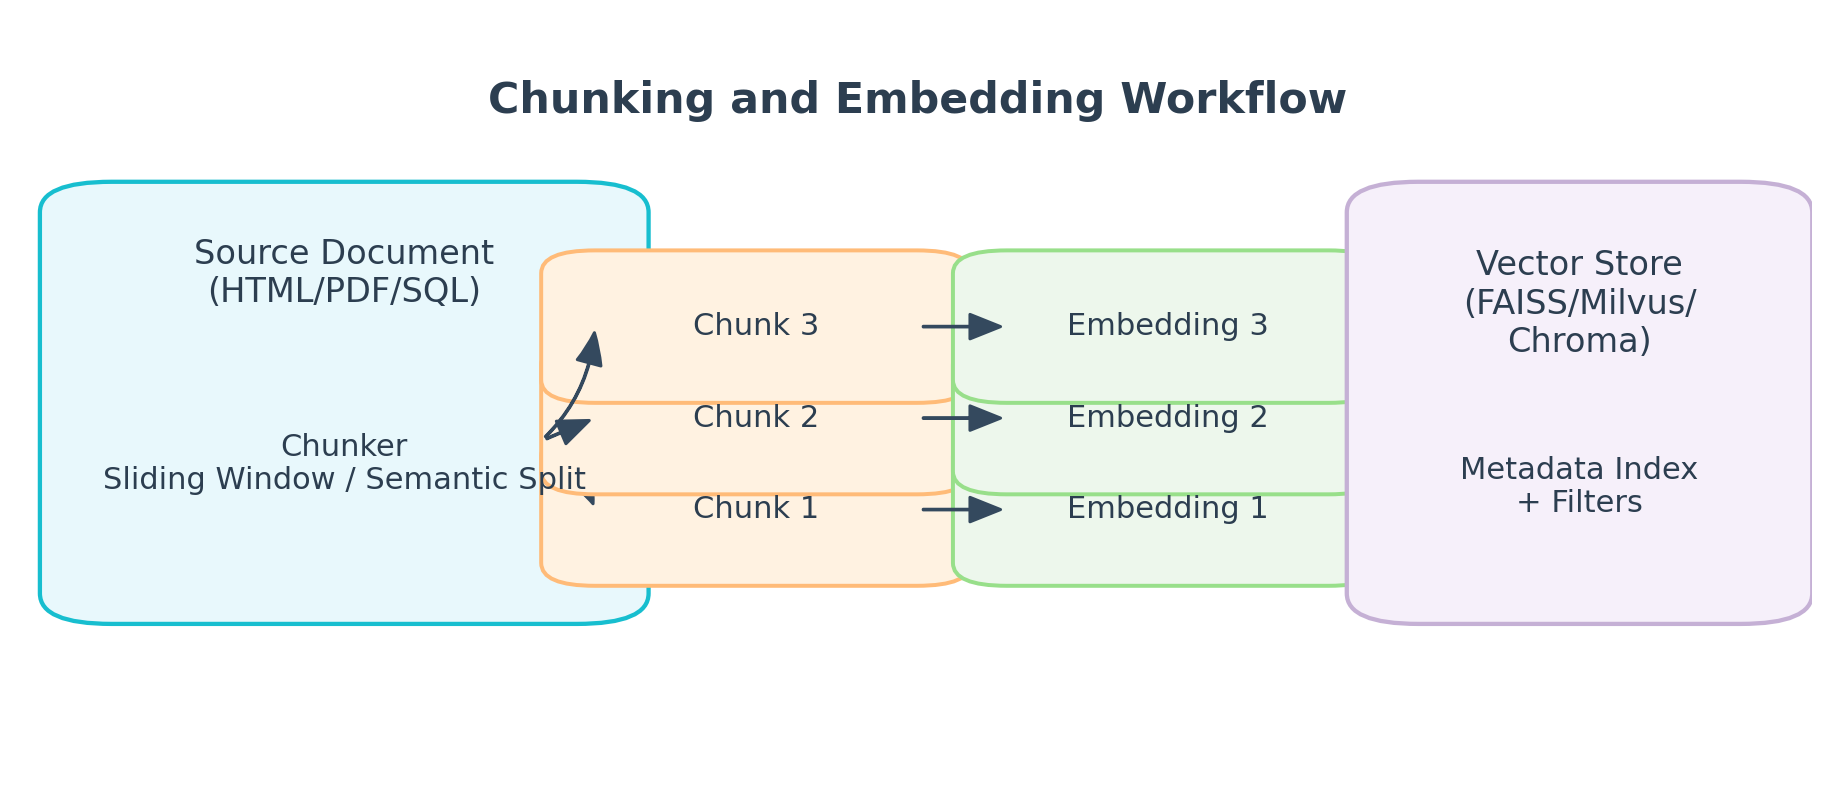
\includegraphics[width=0.9\textwidth]{chunk_embedding.png}
  \caption{Chunking and embedding workflow: raw documents are segmented, encoded, and stored with metadata.}
  \label{fig:chunk_flow_en}
\end{figure}
Key approaches:
\begin{itemize}
  \item \textbf{Fixed windows with overlap:} Ideal for unstructured text; 200--512 token windows with 10--20\% overlap prevent context loss.
  \item \textbf{Semantic segmentation:} Split by sentences, headings, or similarity clustering (TextTiling, sliding cosine similarity).
  \item \textbf{Structured slicing:} Preserve schema for tables, code blocks, knowledge graphs, pairing each chunk with rich metadata.
\end{itemize}

\subsection{Embedding model selection}
\begin{itemize}
  \item \textbf{General-purpose models:} OpenAI \texttt{text-embedding-3-large}, BGE series, E5, and GTR cover multilingual and cross-domain needs.
  \item \textbf{Domain-specific encoders:} Fine-tuned legal, biomedical, or financial models (e.g., bge-law, medembed) boost recall in specialized corpora.
  \item \textbf{Hybrid representations:} Combine dense vectors with sparse retrievers (BM25, SPLADE, ColBERT) to balance lexical and semantic matching.
\end{itemize}

\subsection{Metadata and indexing}
Each embedding is stored alongside metadata:
\begin{itemize}
  \item Document identifiers, chunk offsets, titles, authorship, timestamps, quality scores.
  \item Structured filters (product, geography, access tier) for precise retrieval.
  \item Snippets or abstractive summaries to display in UI and assist the generator.
\end{itemize}

\subsection{Batch embedding example}
\begin{lstlisting}[language=Python,caption={Batch encoding chunks with HuggingFace Transformers}]
from transformers import AutoTokenizer, AutoModel
import torch
import json

tokenizer = AutoTokenizer.from_pretrained("intfloat/multilingual-e5-large")
model = AutoModel.from_pretrained("intfloat/multilingual-e5-large").cuda()

def encode(texts, batch_size=64):
    embeddings = []
    for i in range(0, len(texts), batch_size):
        batch = texts[i:i + batch_size]
        inputs = tokenizer(batch, padding=True, truncation=True, return_tensors="pt").to(model.device)
        with torch.no_grad():
            outputs = model(**inputs)
            emb = torch.nn.functional.normalize(outputs.last_hidden_state[:, 0], p=2, dim=1)
        embeddings.extend(emb.cpu().tolist())
    return embeddings

with open("chunks.jsonl", "r", encoding="utf-8") as f:
    records = [json.loads(line) for line in f]

texts = [r["text"] for r in records]
vectors = encode(texts)

for rec, emb in zip(records, vectors):
    rec["embedding"] = emb

with open("chunks_with_embeddings.jsonl", "w", encoding="utf-8") as f:
    for rec in records:
        f.write(json.dumps(rec, ensure_ascii=False) + "\n")
\end{lstlisting}

\section{Vector Databases: FAISS, Milvus, and Chroma}
\subsection{Feature comparison}
\begin{longtable}{p{3.2cm}p{4cm}p{6cm}}
\toprule
Engine & Highlights & Ideal scenarios \\
\midrule
FAISS & High-performance C++ library with IVF, HNSW, PQ indexes & Single-node deployments with custom optimization \\
Milvus & Cloud-native, distributed, supports vector + scalar filters, CDC & Enterprise-scale, high availability, multi-modal workloads \\
Chroma & Lightweight, built-in persistence, Python-first API & Prototyping, local apps, moderate datasets \\
\bottomrule
\end{longtable}

\subsection{Indexing choices}
\begin{itemize}
  \item \textbf{Flat (exact) search:} Exhaustive dot-product/cosine search; accurate but linear in corpus size.
  \item \textbf{Approximate nearest neighbor (ANN):} IVF, HNSW, ScaNN reduce latency via clustering or graph traversal.
  \item \textbf{Compression:} Product quantization (PQ), optimized PQ (OPQ), or scalar quantization cut memory consumption for billion-scale corpora.
\end{itemize}
Production systems often adopt a two-stage strategy: ANN for coarse retrieval, then re-rank with precise similarity or cross-encoders.

\subsection{FAISS query example}
\begin{lstlisting}[language=Python,caption={Hybrid FAISS search with metadata filtering}]
import faiss
import numpy as np
import pandas as pd

index = faiss.read_index("faiss_ivf_flat.index")
meta = pd.read_parquet("chunk_metadata.parquet")

query = np.load("query_embedding.npy").astype("float32")
k = 8
distances, indices = index.search(query.reshape(1, -1), k)

for dist, idx in zip(distances[0], indices[0]):
    row = meta.iloc[idx]
    if row["language"] != "en":
        continue
    print(f"{row['doc_id']} score={dist:.4f} title={row['title']}")
\end{lstlisting}

\section{Combining RAG with Fine-tuning}
\subsection{Complementary strengths}
\begin{itemize}
  \item \textbf{RAG for freshness:} External knowledge bases update independently of model weights, reducing retraining cadence.
  \item \textbf{Fine-tuning for style/control:} Aligns generation tone, structure, citation behavior, and refusal policy.
  \item \textbf{Joint optimization:} Finetuned generators learn to interpret retrieved passages, disambiguate conflicting evidence, and quote precisely.
\end{itemize}

\subsection{Integration patterns}
\begin{itemize}
  \item \textbf{Instruction tuning + RAG:} Tune the base model on instruction datasets, then feed retrieved context during inference.
  \item \textbf{Retriever tuning:} Train embedding models with contrastive loss (e.g., InfoNCE) using curated positive/negative pairs.
  \item \textbf{Generator tuning:} Supervised fine-tuning or DPO on $(q, evidence, answer)$ triples to reward faithful citations.
  \item \textbf{End-to-end systems:} Architectures like RETRO, Atlas, and HyDE co-train retrieval and generation components.
\end{itemize}

\subsection{Training data assembly}
\begin{itemize}
  \item \textbf{Triplets $(q, d^+, d^-)$:} Hard negatives from BM25 or ANN improve discriminative power of retrievers.
  \item \textbf{Evidence attribution:} Annotate which passages support each answer sentence for supervised citing.
  \item \textbf{Self-generated data:} Let the model answer with retrieved context, score outputs with verifiers, and retain high-quality samples.
\end{itemize}

\subsection{Evaluation matrix}
\begin{longtable}{p{3cm}p{3cm}p{4cm}p{4cm}}
\toprule
Category & Metric & Focus & Tools \\
\midrule
Retrieval & Recall@k, nDCG, MRR & Coverage and ranking quality & BEIR, msmarco eval, LlamaIndex eval \\
Generation & BLEU, ROUGE, factuality scores & Fluency and truthfulness & GPT-judge, FactScore, QAG \\
Citation & Precision@k (citations), hallucination rate & Grounding fidelity & Heuristic citation checkers, regex audits \\
End-to-end & Human ratings, task success, business KPIs & User satisfaction and impact & A/B testing frameworks, analytics dashboards \\
\bottomrule
\end{longtable}

\section*{Operational recommendations}
\begin{itemize}
  \item Enforce structured prompts that label retrieved snippets and request explicit citations or confidence scores.
  \item Schedule periodic index refreshes and monitor drift between embeddings, documents, and generator behavior.
  \item Maintain unified evaluation suites covering retrieval and generation to detect regressions quickly.
  \item Instrument observability for retrieval hit rate, answer accuracy, safety issues, and latency across the pipeline.
\end{itemize}

\section*{Further reading}
\begin{itemize}
  \item Lewis et al. ``Retrieval-Augmented Generation for Knowledge-Intensive NLP Tasks.'' NeurIPS, 2020.
  \item Izacard et al. ``Retrieval in the Contrastive Learning Era.'' arXiv, 2022.
  \item Gao et al. ``Condenser: a Pre-training Architecture for Dense Retrieval.'' EMNLP, 2021.
  \item Chen et al. ``Atlas: Few-shot Learning with Retrieval Augmented Language Models.'' ICML, 2022.
  \item Yu et al. ``Fine-Tuning Language Models with Knowledge Graph Retrieval.'' ACL, 2023.
\end{itemize}

\end{document}

